\documentclass[11.5pt]{sig-alternate} % sets document style to sig-alternate
% packages
% typesetting
% \usepackage{dirtytalk} % can be used to typset quotes easier, automatically sets correct quotation marks with \say{content}
% \usepackage{hanging} % hanging paragraphs with \hanging, like in references. doesn't translate to HTML
\usepackage[defaultlines=3,all]{nowidow} % avoid widows
\usepackage[pdfpagelabels=false]{hyperref} % produce hypertext links, includes backref and nameref
\usepackage{xurl} % defines url linebreaks, loads url package
\usepackage{microtype} % better typography
% \usepackage[super]{nth} % easily create superscript ordinal numbers with \nth{x}
% \usepackage{textcomp} % for better tildes
% \newcommand{\texttildemid}{\raisebox{0.4ex}{\texttildelow}}
% layout
% \usepackage{enumitem} % control layout of itemize, enumerate, description
\usepackage{fancyhdr} % control page headers and footers
% \usepackage{float} % improved interface for floating objects, adds H float
% \usepackage{multicol} % intermix single and multiple column pages
% \textgreek % typeset greek letters in text mode
% language
\usepackage[utf8]{inputenc} % accept different input encodings
\usepackage[english]{babel} % multilanguage support
% misc
\usepackage{graphicx} % builds upon graphics package, \includegraphics
%\usepackage{lastpage} % reference number of pages
\usepackage{xcolor} % color extensions
\usepackage[backend=biber, style=apa]{biblatex} % sophisticated bibliographies % necessary for HTML to display author info and date on abstract page
\usepackage{csquotes} % advanced quotations, makes biblatex happy
\usepackage{authblk} % support for footnote style author/affiliation
% tables and figures
%\usepackage{array} % extend array and tabular environments
\usepackage{caption} % customize captions in figures and tables (rotating captions, sideways captions, etc)
%\usepackage{cuted} % allow mixing of \onecolumn and \twocolumn on same page
\usepackage{multirow} % create tabular cells spanning multiple rows
%\usepackage{subfigure} % deprecated, support for manipulation of small figures
\usepackage{tabularray} % better table construction, does not translate to HTML
%\usepackage{wrapfig} % allows figures or tables to have text wrapped around them
% dummy text
%\usepackage{blindtext} % blind text dummy text
%\usepackage{kantlipsum} % Kant style dummy text
\usepackage{lipsum} % lorem ipsum dummy text
\usepackage{calc}% so we can do inline math within \setlength
\usepackage{enumitem}

\pagestyle{fancy} % sets pagestyle to fancy for fancy headers and footers
% allows the header to take the full width of the page https://www.reddit.com/r/LaTeX/comments/awtrb2/how_to_you_make_the_headerfooter_extend_the/
\newlength{\oddmarginwidth}
\setlength{\oddmarginwidth}{1in+\hoffset+\oddsidemargin}
\newlength{\evenmarginwidth}
\setlength{\evenmarginwidth}{\evensidemargin+1in}
\fancyhfoffset[LO,RE]{\oddmarginwidth}
\fancyhfoffset[LE,RO]{\evenmarginwidth}

% header and footer
% modern way to set header image
\renewcommand{\headrulewidth}{0pt} % defines thickness of line under header
\renewcommand{\footrulewidth}{0pt} % defines thickness of line above header
\setlength\headheight{80.0pt} % sets height between top margin and header image, effectively moves page contents down
\addtolength{\textheight}{-80.0pt} % seems to affect the lower height. maybe only works properly if footer numbers enabled?
\fancyhf{}
\fancyhead[CE, CO]{
\includegraphics[width=\pdfpagewidth]{headerImage.png}}

\hypersetup{colorlinks=true,urlcolor=blue} % sets link color to blue
\urlstyle{same} % sets url typeface to same as rest of text

% set caption and figure to italics, label bold, left align captions, does not transfer to HTML
\captionsetup{labelfont=bf, font={large, it}, justification=raggedright, singlelinecheck=false}
\renewcommand\theContinuedFloat{\alph{ContinuedFloat}} % has something to do with subfigures... don't remember why i used it

%this next bit is confusing, but essentially changes the width of the abstract. Seems to have been copied from this https://tex.stackexchange.com/questions/151583/how-to-adjust-the-width-of-abstract
\let\oldabstract\abstract
\let\oldendabstract\endabstract
\makeatletter %changes @ catcode to enable modification (in parsep)
\renewenvironment{abstract} %alters the abstract environment
{\renewenvironment{quotation}%
               {\list{}{\addtolength{\leftmargin}{1em} % change this value to add or remove length to the the default ?
                        \listparindent 1.5em%
                        \itemindent    \listparindent%
                        \rightmargin   \leftmargin%
                        \parsep        \z@ \@plus\p@}%
                \item\relax}%
               {\endlist}%
\oldabstract}
{\oldendabstract}
\makeatother %changes @ catcode to disable modification

% checks
% italics 
% links
% dashes
% tildes
\begin{document}

\title{A Summer Class Exploring Computer Science with Educators of Deaf and Hard of Hearing Students}

\author[1]{\large \color{blue} Meghan L. McSherry} % make sure there are no spaces after the author's name
\author[1]{\large \color{blue} Becca A. Leininger}
\author[1]{\large \color{blue} Maria L. Johnson}
\author[1]{\large \color{blue} AnnMarie P. Thomas}
\author[2]{\large \color{blue} Susan Outlaw}
\author[1]{\large \color{blue} Douglas C. Orzolek}

\affil[1]{Playful Learning Lab, University of St. Thomas}
\affil[2]{Metro Deaf School}
\toappear{} % the sig.alternate document type includes a copyright warning that appears at the bottom of the first page. This makes that not appear/be empty. Don't ask my why it's there in the first place /shrug

\maketitle % prints article title
\begin{@twocolumnfalse} 
\begin{abstract}
\item %the abstract is a quotation and a list, so this must be an item
\begin{large}
\textit{The purpose of this research project was to design, deliver, and informally assess the content and methodology of an introductory online course for the educators of Deaf and Hard of Hearing students (N=20) that focused on the block-based coding language, Scratch. Prior work by The Playful Learning Lab examined various STEM resources and their effect on student perception of STEM topics and content retention when utilized for Deaf and Hard of Hearing K-12 students. Previous research has shown that computer science and programming resources and curricula available today are not fully accessible for Deaf and Hard of Hearing K-12 students. Educators and teachers are faced with creating adaptations themselves, often limited by time constraints (Ladner, 2020). The purpose of the summer 2023 “Playing with Coding” course was to provide the background knowledge and content to educators of Deaf and Hard of Hearing students so they are able to explore the possibility of teaching the programming language in their own classrooms. Through our research and participant survey reflections, we hoped to determine effective methods and resources that educators can use to successfully teach the Scratch programming language to Deaf and Hard of Hearing students.}

\item Keywords: Computer Science, Deaf, Professional Development
\end{large}     
\end{abstract}
\end{@twocolumnfalse}

%% AUTHOR INFORMATION
\textbf{*Corresponding Author, Meghan L. McSherry}\\ % corresponding author
\href{mailto:mcsh2623@stthomas.edu}{mcsh2623@stthomas.edu} \\ % author email
\textit{Submitted Mon Jan 22} \\ % submitted date
\textit{Accepted Fri Sep 13} \\ % accepted date
\textit{Published Online Wed Dec 4} \\ %published online date
\textit{DOI: 10.14448/jsesd.16.0003} \\ % doi
\pagebreak 
\clearpage % both needed to go to next page

\begin{large}
\section*{INTRODUCTION}

Recent trends in education have focused on STEM learning and activities in hopes these approaches will help meet job demands and the need to advance society (Gardner, Glassmeyer, and Worthy, 2019). Like all other areas of learning, it is important that STEM educators keep informed of trends and issues related to both the job market as well as the best approaches to helping students develop their skills. One of the key means of helping educators grow and remain informed is through professional development opportunities which can be offered through a variety of means: in-person experiences, online classes, college coursework, and several other means. Perhaps more importantly, research suggests that teachers who continue to grow and learn through professional development help their students achieve at higher levels—and this is especially true in STEM areas (Wojnowski and Pea, 2013).

Educators serving students who are Deaf or Hard of Hearing serve a population that is very unique and who hold many special needs. However, specific professional development that is specifically aligned with supporting teachers who teach this population is limited and often difficult to access (Tiggs, 2021). Tiggs further suggested that (2020):

\begin{quote}
    … building a culture that encourages educators of students who are deaf or hard of hearing to take charge of their learning needs could assist training providers at the pre-service and in-service levels to better support those educators in personalizing their professional development. (ii)
\end{quote}

According to Long and Kowalske (2022), the Deaf and Hard of Hearing community is underrepresented in the STEM community which they believe may be the direct result of the lack of professional development that is available to the educators who work with Deaf and Hard of Hearing Learners. They believe that one of the goals of those who support teachers of Deaf and Hard of Hearing students interested in STEM areas should be “to build confident communities of educated advocates in STEM academia, who are equipped with knowledge and resources on how to best support their D/HH students” (p. 291). This project attempted to do just that.

The Playful Learning Lab (PLL) is an interdisciplinary, student research lab at the University of St, Thomas located in Saint. Paul, Minnesota that focuses on encouraging education in PK-12 students through play. PLL student researchers come from diverse academic backgrounds, with majors such as engineering, education, computer science, and biology. The PLL collaborates with community partners like Metro Deaf School, Twin Cities Trapeze, and The Minnesota Children’s Museum on projects such as OK GO Sandbox (Schumacher et al., 2020), Circus Science (Roche et al., 2020), and The PLAYground (Monson et al., 2020). 

The Playful Learning Lab has been collaborating with Metro Deaf School (MDS), a Deaf charter school in Saint Paul, Minnesota, for over 9 years through a variety of projects including teacher workshops, classroom curriculum support, and by creating many opportunities for the students of MDS to learn about STEAM concepts through play (Kasper et al., 2016; Monson et al., 2020). The PLL hosted a workshop at MDS during the summer of 2022 to begin the creation of a computer science network of educators from Deaf schools and schools with Deaf programs. This in-person workshop was hosted for MDS educators to explore the basics of Scratch, a block-based programming language intended for children, and how it could be applied in their classrooms. Members of the Playful Learning Lab worked directly with MDS teachers through the spring 2023 school year to incorporate LEGO Spike, KIBO, Scratch, and  Scratch Jr, into their classrooms.

Many computer science and programming resources and curricula available today are not fully accessible for Deaf and Hard of Hearing students. The resources tend to be created with the general needs of hearing students in mind, forcing educators of Deaf and Hard of Hearing students to adapt the material on their own while taking into account their students’ individual needs (Ladner, 2020). For example, some curriculum alterations include creating more visual-oriented lesson plans and additional exercises that orient students to software or materials. Educators often lack sufficient time to do this, so there is an urgent need for available and accessible computer science educational resources created specifically for Deaf and Hard of Hearing K-12 students. Educators of these students suggest that academic content should be visual-oriented and keep in mind that their students benefit from both English and ASL formats. ASL interpretation is ideal for educational resources for Deaf and Hard of Hearing K-12 students, but due to time constraints and the cost of hiring interpreters, this is not often possible for schools and programs to accommodate. Without these accommodations and without access to educational resources specifically intended for Deaf and Hard of Hearing K-12 students, their educational needs can go unfilled (Reinholz et al., 2021). This project intended to address this disparity.

Based upon its experience developing visual-oriented computer science resources for Deaf and Hard of Hearing students, the Playful Learning Lab used the visual and block-based coding platform Scratch as an accessible means of computer science education. The programming language is free online at scratch.mit.edu, and it is designed to offer kids a fun, manageable, and creative entry into computer programming. There is limited literature available on using Scratch to educate Deaf and Hard of Hearing K-12 students, so this research aimed to address a gap in the literature by creating accessible computer science resources. By exploring the effectiveness of using Scratch alongside ASL interpreted lesson plans, we hoped to enhance Deaf and Hard of Hearing students’ understandings of broad STEAM concepts. 

\section*{COURSE DEVELOPMENT}

\subsection*{Course Goals}

With the aim of working towards addressing the inequities in Computer Science education for Deaf and Hard of Hearing students, the PLL and MDS combined efforts and received a grant from Google that would fund these three goals:

\begin{itemize}[parsep=4em]
    \item The completion of an assessment of the current state of computer science and computational thinking programs and content at US Deaf schools and schools with Deaf programs, with a focus on elementary and middle school classes; 
    \item The co-creation (with elementary and middle school teachers) and assessment of research based Computer Science units for Deaf and Hard of Hearing elementary and middle school students;
    \item The creation of a network of teachers from Deaf schools (and schools with Deaf programs) discussing computer science curriculum for Deaf, and Hard of Hearing children.
\end{itemize}

The PLL’s 2022 summer workshop was the beginning of the creation of a network of teachers from Deaf schools and schools with Deaf programs. The goal of creating this network was to strengthen the educators’ computational thinking literacy and provide them with the skills and resources to do the same with their own  students. Due to the success of this workshop, the Playful Learning Lab wanted to expand this network even further to create a larger cohort of teachers. Our goal was to determine the most effective methods and resources that educators could use to successfully teach the Scratch programming language to Deaf and Hard of Hearing students. The PLL’s previous research discovered that computer science and programming resources and curricula available today are not fully accessible for Deaf and Hard of Hearing students. As noted earlier, educators often have to figure out how to adapt materials on their own and often lack the time and support to do so (Ladner, 2020). With this in mind, the purpose of the summer 2023 workshop, entitled “Playing with Coding,” was to design, deliver, and assess the content and methodology of an introductory course focused on the block-based coding language, Scratch, for educators of Deaf and Hard of Hearing students. 

\subsection*{Planning Playing with Coding}

With the intent of creating a network of educators that could build on their coding literacy, the PLL planned for the workshop to include numerous means of communication and multiple activities aimed at different coding learning strategies. The summer before “Playing with Coding,” PLL members engaged in the activities of available online curriculums to practice the Scratch programming language including Harvard’s “Getting Unstuck” curriculum. This curriculum broke down the lessons into modules themed around individual coding concepts such as loops and broadcasting. It included videos and slides and we found it to be an effective way for our team members to practice using the Scratch programming language and we decided to build on this approach for our own class. After corresponding with Harvard’s Creative Computing Lab, the PLL was given permission to utilize the videos and coding concepts from “Getting Unstuck” as a means to create the foundation of our “Playing with Coding” curriculum. 

The Playful Learning Lab designed “Playing With Coding” as an eight-week, introductory course with a new module being published weekly. Each module focused on one or two coding concepts through videos, handouts, and specific online activities. In addition to eight weekly modules, two resource modules were developed and provided. One introduced the PLL and our work as well as  how to contact us for support or help, and the other resource module contained bonus materials for the consideration of further Scratch application. To encourage community, discussion boards were included within the modules of the class. Here, the educators could introduce themselves, share ideas and projects, engage with one another, and ask for additional support.  

Educators of Deaf and Hard of Hearing students were recruited to participate in our course through the same outreach we conducted to determine the current state of computer science and coding content being taught to Deaf and Hard of Hearing students around the United States. When reaching out to these schools and programs, we included a flier detailing the course as an introduction to Scratch, so the educators can learn how Scratch works before bringing it to their own students and schools. The advertisement emphasized that “Playing With Coding” was designed for educators of Deaf and Hard of Hearing students who were new to Scratch, and that they would earn a \$250 honorarium when they completed the course. A total of twenty teachers agreed to be engaged in the workshop and only one indicated that they had a background in coding. The participants primary area of teaching were as follows: three focused in the area of working with Deaf/Hard of Hearing; two were language arts; five were from the Science/STEAM areas; six indicated general education; and four indicated occupational therapy/life skills.

Because many of the teachers enrolled in the class were Deaf or Hard of Hearing themselves and with the hope that the educators in “Playing with Coding” would use the provided resources in their classrooms, side-by-side American Sign Language (ASL) interpretations were incorporated into every video throughout the workshop. The PLL also created resource documents with high contrast versions to make them accessible for those who have low vision, are blind, or are colorblind.

\section*{METHOD}

\subsection*{Weekly Module Structure}

Throughout the summer workshop, one module was released each week using a similar structure. The modules were designed so participants could work through each step of the module in a carefully developed sequence of learning. The modules started with watching videos, learning a new coding concept, debugging a coding issue, creating a personal project, and participating in discussion boards to consider and address potential classroom applications. “Bonus” videos were also included to show how Scratch was being used by other educators. These “classroom application videos” suggested ways that Scratch could  be shared with students. For example, one bonus video featured Sandy Culpepper, a middle school teacher at Metro Deaf School, in which she explained how she utilized Scratch as a learning tool. Another video showed Dr. Karen Brennan, the Director of Harvard's Creative Computing Lab that developed the “Getting Unstuck” curriculum. In her video, she discussed the benefits of practicing computational thinking skills with K-12 students.

Scratch contained tutorial videos on their website, but only the “Getting Started” video included ASL interpretation. Some coding concepts taught in the course included parallelism, loops, and variables, which correlated to lessons in the “Getting Unstuck” curriculum (Brennan et al., 2021). In our course, the PLL explained these concepts through a variety of methods to keep the course participants engaged and to introduce them to different methods of teaching this material to their students. 

The “Getting Unstuck” curriculum included several activities that were titled “Debug Its” that engaged the learner in the process of debugging codes. “Debugging” is a term used by programmers to describe the process of combing through their code to find and resolve “bugs”—issues, mistakes, or problems to fix to make sure the program works as intended. This process can also be helpful in learning computer science because it requires the careful reading and interpretation of code. In “Playing With Coding,” teachers were given three different Scratch projects adapted from “Getting Unstuck.” As intended, the codes did not work correctly and the educators were asked to “debug” them so they would run as desired. There is never one correct answer when resolving coding issues, so these activities challenged the course participants to creatively problem-solve.

The development of creative problem-solving skills was another important aspect of the workshop. We found that the weekly-assigned personal projects exhibited the most creativity from the course participants. For example, the “Create a Maze!” project gave the educators a “Maze Starter,” created by the team at Scratch, asked participants to develop an interesting maze and apply what they had learned. Specifically, we encouraged them to add more obstacles, create new levels, keep score, or try anything else they desired. Throughout these experiences, we aimed to provide teachers with a space to interact with each other and share implementation ideas through discussion boards. Through these discussion boards, the educators posted multiple creative means for applying Scratch to classrooms. For example, many noted that Scratch could be used in place of an essay or slide show, as it makes for a less language-heavy presentation tool.

\subsection*{Conducting “Playing with Coding”}

There were various organizational aspects of the workshops that became focal points of conducting “Playing with Coding.” First, offering soft timeline requirements for completing modules made the workshop more manageable for participants to work through the materials at their own pace. PLL members dispatched emails at the beginning of each week stating that the next module was now available, but there was no designated timeframe in which assignments needed to be completed. Some participants turned in assignments on a near-weekly basis, while others began their work later in the summer.

Second, we found that grading and providing feedback on the assignments completed by the educators became a crucial way to maintain engagement between ourselves as the instructors and the “Playing With Coding” participants. Those dialogues helped us to adjust subsequent lessons so that we could properly sequence their learning of the coding concepts. Because of the soft timeframe for completing modules, we ensured that assignment submissions were reviewed promptly to provide feedback and mark the assignments as complete. At the end of the course, teachers were required to have all assignments turned in before submitting an invoice for their honorarium.

Third, to make the course as flexible as possible, we provided participants with a variety of means to contact the “Playing With Coding” instructors if they required assistance with anything throughout the summer. We know that teachers often have hectic summers, and because of that, we attempted to ensure that participating in the workshop felt easy and comfortable. We offered weekly personalized email reminders, weekly discussion boards, personal and regular comments on submissions, and set up personal Zoom meetings so the participants could ask questions as needed.

Finally, another way the “Playing With Coding” staff connected with the participants was by mailing them surprise care packages. Each educator received a kit with a Makey Makey and some Squishy Circuits dough, both of which are STEAM tools for children that make programming a more tactile experience. We also included a bonus module on the course with more info on how to use these products with their students.

\section*{QUANTITATIVE AND QUALITATIVE RESULTS}

Because the primary focus of this project was with the development of the modules and learning  opportunities, informal surveys were developed to gather information about the impact and helpfulness of the workshop. At the end of each of the “Playing With Coding” modules, optional surveys were included to evaluate how effective the curriculum was at teaching that week’s coding concept and to assess how we could better support the educators in the workshop. From these surveys, it was determined that most of the respondents viewed the content as somewhat difficult, yet most felt confident in the skills they developed after going through that module and that they were supported by us throughout the process. Of  the resources included in each module, the results indicated that the videos that included ASL interpretation were most often used and regarded as helpful in learning the coding concepts. We also learned that the optional, written lessons were rarely used by the participants. While we had hoped for more responses to the surveys, overall they aided us in determining how effective each activity was as well as how supported the educators felt in their learning process.

When course participants were asked “How would you rank the difficulty of this week’s module?” most responses (N=12) indicated that the modules were “somewhat difficult.” Six respondents answered, “neither easy nor difficult” and two answered, “somewhat easy.” (See Figure 1.)

\begin{figure}[th]
    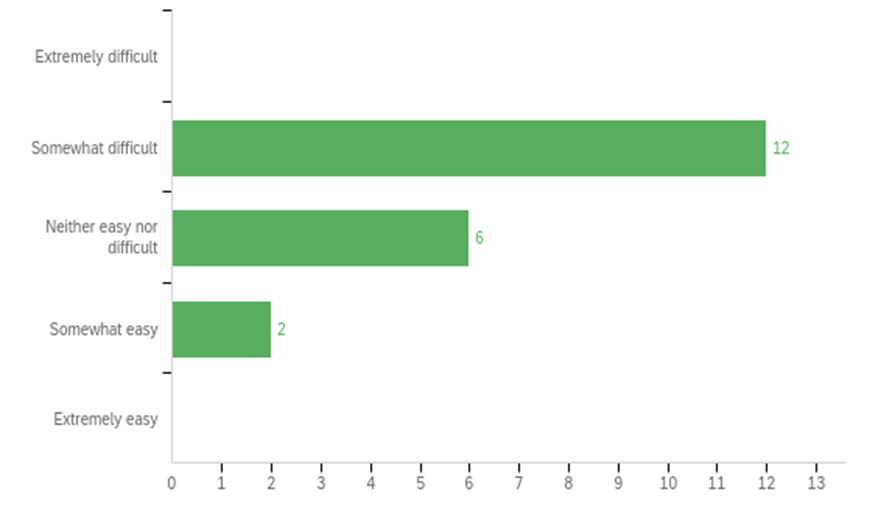
\includegraphics[width=\linewidth]{images/fig1.png}
    \caption{Educators’ Difficulty Ratings for Weekly Modules}
    \label{Figure 1}
\end{figure}

Participants were also asked at the end of module surveys “How confident in this week’s coding concept(s) do you feel after completing this module?” (See Figure 2.) Most respondents (N=11) indicated that they felt “moderately confident” in their understanding of that week’s coding concept, while two  felt “extremely confident,” 5 responses selected “somewhat confident,” and two said “somewhat unconfident.”

\begin{figure}[th]
    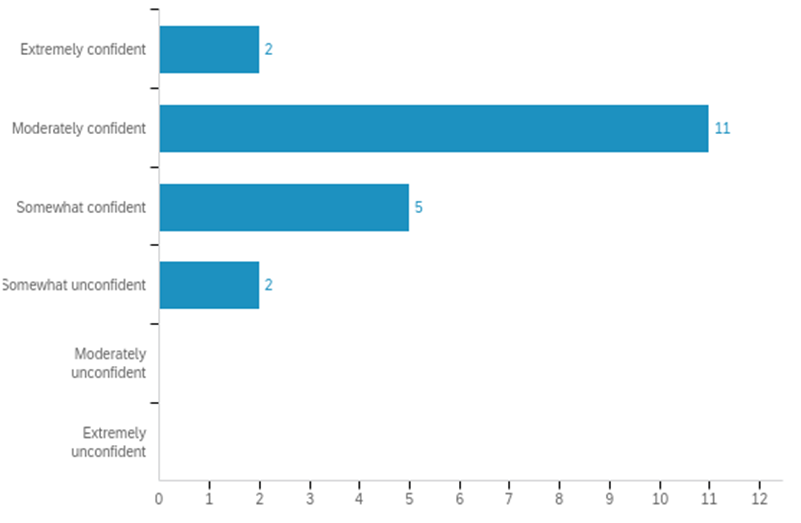
\includegraphics[width=\linewidth]{images/fig2.png}
    \caption{Educators’ Confidence Level Ratings in Understanding of Weekly Coding Concept(s)}
    \label{Figure 2}
\end{figure}

Respondents were also asked, “How supported did you feel in completing this week’s module?.” Here the educators (N=9) indicated that they felt “very supported” in completing that week’s module, seven answered they felt “moderately supported,” and four felt “somewhat supported.” (See Figure 3.)

\begin{figure}[th]
    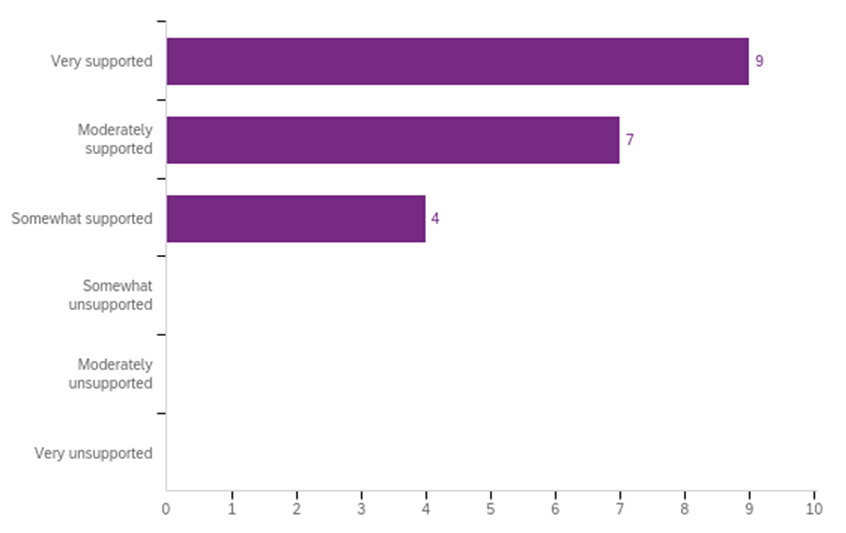
\includegraphics[width=\linewidth]{images/fig3.png}
    \caption{Educators’ Perceived Support in Completing Weekly Modules}
    \label{Figure 3}
\end{figure}

Survey respondents were also asked if the resources marked as  “Watch,” “Read,” and “Additional Classroom Resources” were helpful, unhelpful, or went unused in learning Scratch. If resources were helpful, respondents answered “Yes” and “No” if they found them to not be helpful. The answer option “Didn’t use it” indicated that that respondent did not utilize that resource. There were twenty responses to this question. Out of the resources that the responses indicated “Yes” to being helpful, twenty indicated the “Read” resources, seventeen selected the “Watch” resources, and nine posited that the “Additional Classroom Resources” were helpful to them. Respectively, eleven and three respondents indicated that the “Watch” and “Read” were not helpful to them. No one selected that they did not use any of these resources. (See Figure 4.)

\begin{figure}[th]
    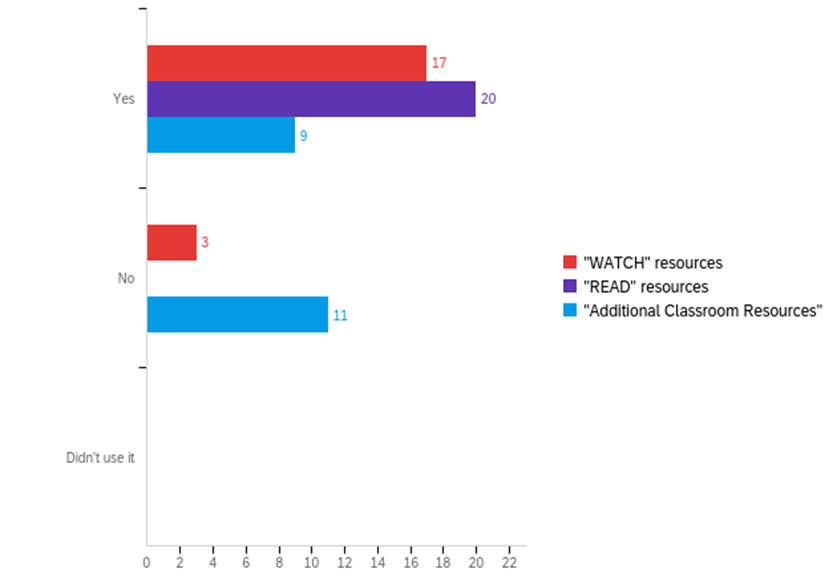
\includegraphics[width=\linewidth]{images/fig4.png}
    \caption{Educator Feedback on Effectiveness of Coding Educational Resources}
    \label{Figure 4}
\end{figure}

\section*{RESOURCES PRODUCED}

One of “Playing With Codings” goals was to support multiple learning types. After learning that there were limited programming and coding educational resources available for Deaf and Hard of Hearing K-12 students, we created and outsourced a wide variety of learning resources. As noted earlier, we used videos and lesson plans from Harvard’s “Getting Unstuck” curriculum but added ASL interpretations to assist in the learning. We also programmed multiple debugging exercises that we adapted for Deaf and Hard of Hearing individuals. For example,  Scratch programs often included sound which allowed us to adjust the learning experiences. We also had multiple requests from the participants to make handouts including the learning materials available to them. Many of them wanted to return to the Scratch educational resources later or use them in their own classrooms. In response to these requests, we compiled an ASL resource document and a handout that includes the resources from “Getting Unstuck” (See Appendix A.).

\section*{LIMITATIONS}

A primary limitation for this project was the small number of participants and the lower-than-expected engagement levels. As mentioned earlier, educators were recruited through a flier attached to the end of a survey assessing the state of computer science programs at Deaf schools and schools with Deaf programs in the United States. This survey received few responses and, in turn, even fewer recruitments for “Playing With Coding.” As a result, most participants were recruited through personal connections and through the PLL’s previous partnership with the Metro Deaf School. In total, only twenty people enrolled in the course, ten of the twenty who enrolled participated in some way, and four completed the entirety of the workshop modules. These numbers reflected not only the low participant number, but the low participation levels of the people who were enrolled. Of the educators who completed the class, no one requested to schedule a meeting with instructors during the workshops and very few reached out with questions or comments through the available discussion boards or email.

With very few participants finishing “Playing With Coding,” the course and survey results were limited by the small sample size. We suspect this was because teachers were already preoccupied throughout the summer, and because the workshop provided very flexible timelines for completing the modules. However, we believe there are still opportunities to increase engagement if “Playing With Coding” were to be offered again in the future. For example, we offered virtual meetings with the educators but none were requested. Scheduling some optional meetings or open office hours throughout the workshop might help the teachers feel more engaged and encourage more of them to complete the course.

\section*{CONCLUSION}

“Playing With Coding” did not yield sufficient results in evaluating the effectiveness of the curriculum, but the course did succeed in producing several accessible, educational computer science resources to aid in the efforts to eliminate disparities in STEAM education for Deaf and Hard of Hearing K-12 students. In addition to these resources, we gained valuable insights into what type of educational resources the educators of Deaf and Hard of Hearing K-12 students need to support their own learning process and those of their students. Despite our course surveys receiving limited responses, it is evident that educators benefit from including multiple educational mediums such as videos, handouts, and activities. Various accessible options are necessary in implementing an effective computer science curriculum and this study further supported that contention. Regarding the future direction of “Playing With Coding,” there are numerous possibilities available to further our research. For example, we could as run the course again with a better participant recruitment strategy including publicizing the course more widely and providing a promise for access to additional resources. Regardless of any next steps “Playing With Coding” will take, the Playful Learning Lab will continue to use its accessible programming educational resources to grow and support the impact of playful education for the purposes of eliminating educational disparities for Deaf and Hard of Hearing K-12 students.  

\section*{ACKNOWLEDGEMENTS}
The authors would like to thank their Playful Learning Lab colleagues and the staff at Metro Deaf School. The work was made possible through support from the Google Computer Science Education Research awards program, and the Scratch Foundation.

\end{large}
\clearpage
\section*{REFERENCES}\par 

\leftskip 0.25in
\parindent -0.25in % create hanging indents for references. if article has content after references, set leftskip and parindent to 0

B. Kasper, A. Haugh, N. Kasper, B. Gunderson, AM. Thomas, and D. Besser. (2016) \textit{Design, Implementation, and Assessment of an After-School Engineering Program for Deaf Students}. Proceedings of the ASEE Annual Conference. New Orleans, LA. 

Brennan, K., Balch, C., \& Chung, M. (2014). \textit{Creative computing: A design-based introduction to computational thinking}. Harvard Graduate School of Education. \url{https://creativecomputing.gse.harvard.edu/guide/}

Brennan, K., Haduong, P., Williamson, M. A., Peters, L., Smolevitz, S., \& Yu, B. (2021). \textit{Getting unstuck: An intermediate Scratch curriculum to support design studio culture in the classroom}. Creative Computing Lab. Retrieved from \url{https://gettingunstuck.gse.harvard.edu}

Gardner, K., Glassmeyer, D., \& Worthy, R. (2019, April). Impacts of STEM professional development on teachers' knowledge, self-efficacy, and practice. In \textit{Frontiers in Education} (Vol. 4, p. 26). Frontiers Media SA.

Ladner, R. E., Stefik, A., Naumann, J., \& Peach, E. (2020). \textit{Computer science principles for teachers of deaf students. 2020 Research on Equity and Sustained Participation in Engineering, Computing, and Technology (RESPECT)}. \url{https://doi.org/10.1109/respect49803.2020.9272432}

Leininger, Becca; Yang, Christina; Quinn, Makayla; Jalkio, Jeffrey; Bahajry, Rahaf; Ingabire, Mellissa; and Thomas, AnnMarie (2023). \textit{An Introductory Course in Electrical Circuits and Coding for Deaf and DeafBlind Middle School Students. Journal of Science Education for Students with Disabilities}: Vol. 26 : Iss. 1, pp. 1-10, Article 8. DOI: 10.14448/jsesd.15.0008 Available at: \url{https://repository.rit.edu/jsesd/vol26/iss1/8}

Long, M. R., \& Grunert Kowalske, M. (2021). Understanding STEM Instructors’ Experiences with and Perceptions of Deaf and Hard-of-Hearing Students: The First Step toward Increasing Access and Inclusivity. \textit{Journal of Chemical Education, 99}(1), 274-282.

Monson, E., Schumacher, K., \& Thomas, AM. (2020). \textit{The PLAYground: An online summer camp for deaf and hard of hearing children. Journal of Science Education for Students with Disabilities, 24}(1). \url{https://doi.org/10.14448/jsesd.13.0008}

Reinholz, D. L., \& Ridgway, S. W. (2021). \textit{Access needs: Centering students and disrupting ableist norms in STEM. CBE—Life Sciences Education, 20}(3), es8. 

Tiggs, S. C. (2021). \textit{Perceptions of Professional Development: A Descriptive Study Investigating Learning Opportunities for Teachers of Students Who Are Deaf or Hard of Hearing} (Doctoral dissertation, Regent University).

Wojnowski, B. S., \& Pea, C. H. (2014). Models Approaches. \url{https://static.nsta.org/pdfs/samples/PB322Xweb.pdf}

\clearpage
\leftskip 0in
\parindent 0in % create hanging indents for references. if article has content after references, set leftskip and parindent to 0
\begin{large}

\section*{APPENDIX A}

\subsection*{End of Weekly Module Survey Questions}
Q1. How Confident in this week’s coding concept(s) do you feel after completing this module?

\begin{itemize}
    \item Extremely confident 
    \item Moderately confident 
    \item Somewhat confident 
    \item Somewhat unconfident 
    \item Moderately unconfident 
    \item Extremely unconfident 
\end{itemize}

Q2. Approximately how much time did you spend completing the assignments for this week? 

Q3.
\begin{table}[h]
\begin{tabular}{|l|c|c|c|}
\hline
& \multicolumn{3}{|c|}{Was this resource helpful to you?} \\ \hline
& Yes & No & Didn't use it \\ \hline
“WATCH” resources & \textbullet & \textbullet & \textbullet \\ \hline
“READ” resources & \textbullet & \textbullet & \textbullet \\ \hline
“Additional Classroom Resources” & \textbullet & \textbullet & \textbullet \\ \hline
\end{tabular}
\end{table}

Q4. How supported did you feel in completing this week’s module?

\begin{itemize}
    \item Very supported 
    \item Moderately supported 
    \item Somewhat supported 
    \item Somewhat supported 
    \item Somewhat unsupported 
    \item Moderately unsupported 
    \item Very unsupported 
\end{itemize}

Q5. Did you have to look for any outside resources to complete this week’s module?

\begin{itemize}
    \item Yes
    \item No
\end{itemize}

Q6. How would you rank the difficulty of this week’s module? 

\begin{itemize}
    \item Extremely difficult 
    \item Somewhat difficult 
    \item Neither easy nor difficult 
    \item Somewhat easy
    \item Extremely easy
\end{itemize}

Q7. Were you able to connect with the PLL staff for any questions or confusing content?

\begin{itemize}
    \item Yes
    \item No
\end{itemize}

\clearpage

\onecolumn
\section*{APPENDIX B}
\subsection*{ASL Interpreted Video Handout}


\begin{figure}[hb]
    \centering
    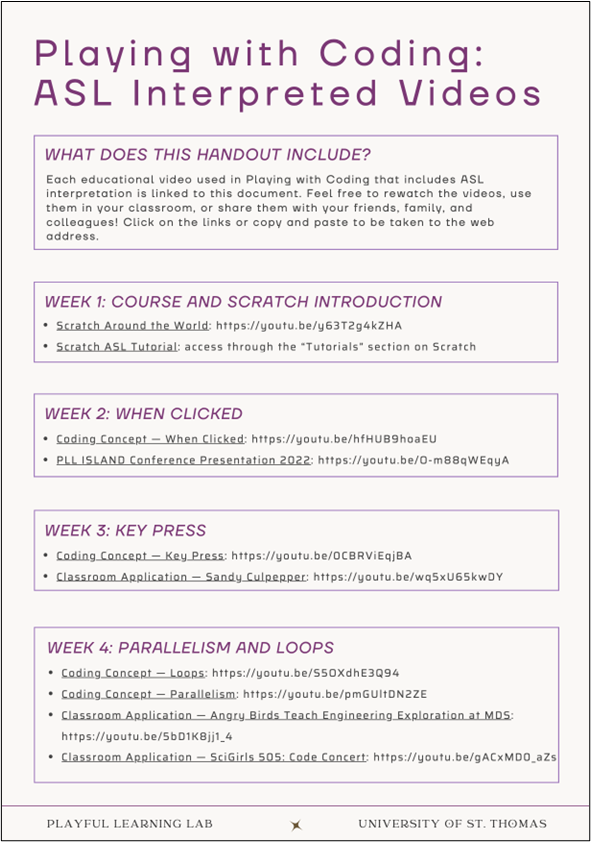
\includegraphics[width=0.62\textwidth]{images/appendix1.png}
    \label{Appendix 1a}
\end{figure}

\begin{figure}[hb]
    \centering
    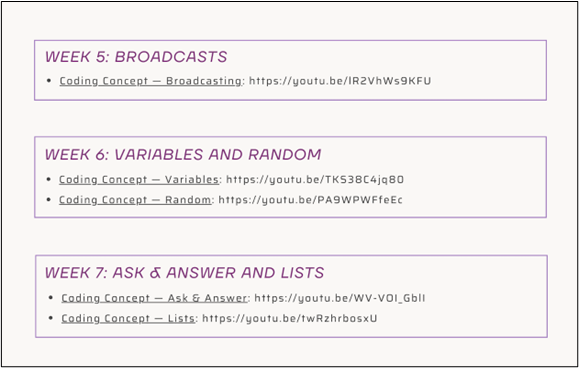
\includegraphics[width=0.62\textwidth]{images/appendix1_b.png}
    \label{Appendix 1b}
\end{figure}

\clearpage

\section*{APPENDIX C}
\subsection*{Getting Unstuck Classroom Guides Handout}


\begin{figure}[hb]
    \centering
    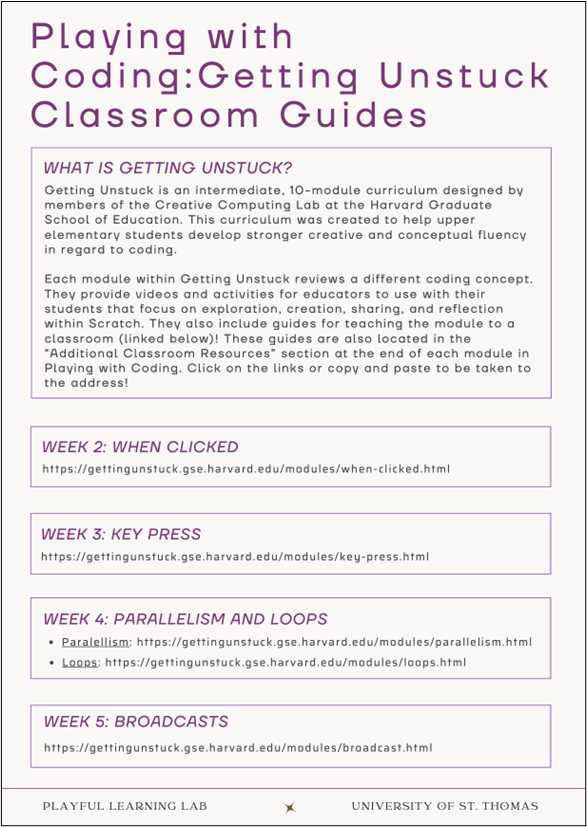
\includegraphics[width=0.62\textwidth]{images/appendix2.png}
    \label{Appendix 2a}
\end{figure}

\begin{figure}[hb]
    \centering
    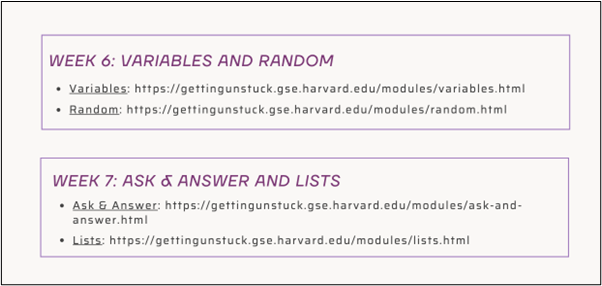
\includegraphics[width=0.62\textwidth]{images/appendix2_b.png}
    \label{Appendix 2b}
\end{figure}

\end{large}
\end{document}
